\documentclass[10pt]{article}
\usepackage{amsmath,amssymb}
\setlength{\oddsidemargin}{0in}
\setlength{\evensidemargin}{0in}
\setlength{\textheight}{9in}
\setlength{\textwidth}{6.5in}
\setlength{\topmargin}{-0.5in}
\usepackage{enumitem}
\usepackage[table]{xcolor}
\usepackage{graphicx}
\usepackage{listings}
\usepackage{float}
\newcommand{\Adv}{{\mathbf{Adv}}}       
\newcommand{\prp}{{\mathrm{prp}}}             
\newcommand{\calK}{{\cal K}}
\newcommand{\outputs}{{\Rightarrow}}                



% Use \textbf{Solution:}\\ to begin your solution.

%%%%%%%%%%%%%%%%%%%%%%%%%%%%%%%%%%%%%%%%%%%%%%%%%%%%%%%%%%%%%%%%%%%%%%%%%%%
\title{\bf Math 151A: Problem Set 2}
\date{4/21/2023}
\author{\bf Owen Jones}

\begin{document}
\maketitle


{\small \textbf{Instructions}:
\begin{itemize}
\item Due on Friday, April 21st by 1:00pm.
\item Late HW will not be accepted.
\item Write down all of the details and attach your code to the end of the assignment for full credit (as a PDF).  
\item If you LaTeX your solutions, you will get $5\%$ extra credit. 
\item (T) are ``pencil-and-paper'' problems and (C) means that the problem includes a computational/programming component. 
\end{itemize}}

%Add \newpage  between problelms if you are using this to LaTex your solutions




%%%%%%%%%%%%%%%%%%%%%%%%%%%%%%%%%%%%%%%%%%%%%%%%%%%%%%%%
\begin{enumerate}[label=\bfseries Problem \arabic*:]

\vspace{1em}
%%%%%%%%%%%%%%%%%%%%%%%%%%%%%%
\item \textbf{(T \& C) Fixed-Point Method}\par 
Consider the fixed-point problem $x=g(x)$ where $$g(x):=\frac{\sin(x)+\cos(x)}{2}.$$ Determine an interval $[a,b]$ such that the fixed-point method converges. Provide the number of iterations necessary to obtain a $10^{-5}$-accurate approximation (using the corollary from class) and perform the calculation to obtain the approximation.\\
\vspace{1em}
\textbf{Solution:}\par 
The maximum and minimum values of $g(x)$ for $x\in[\frac{1}{2},1]$ must occur at the endpoints or when $g'(x)=0$. 
$g(x)$ assumes a minimum at the endpoint $g(\frac{1}{2})\approx0.6785$ and a maximum when the derivative is 0 $g(\frac{\pi}{4})=\sqrt{2}\approx0.7071$.
Thus, $g$ is a continuous function that maps onto itself over the interval $[\frac{1}{2},1]$.
$|g'(x)|$ for $x\in[\frac{1}{2},1]$ assumes a maximum at the endpoint $|g'(\frac{1}{2})|\approx0.1991$, so let $k=0.1991$.
Thus, $|g'(x)|$ is bounded above by a $k$ less than 1.
By Theorem 2.3, a unique fixed point $p$ exists on the interval $p\in[\frac{1}{2},1]$.
Because a unique fixed point $p$ exists and $|g'(x)|\le k<1$ the Fixed Point Theorem states $g(x)$ converges to the unique fixed point for any $p_0\in[\frac{1}{2},1]$. 
It follows we can use corollary 2.5 to find the maximum number of iterations we need to obtain a $10^{-5}$-accurate approximation. 
Using initial estimate $p_0=0.75$, $|p_n-p|\le \frac{k^n}{1-k}|p_1-p_0|=0.0434\frac{(0.1991)^n}{0.8009}\le0.0542(0.1991)^n\le10^{-5}$.
This implies $n\ge -\frac{5+\log(0.0542)}{\log(0.1991)}\approx 5.327$.
Hence, we are guaranteed to obtain a $10^{-5}$-accurate approximation within 6 iterations. 
\begin{figure}[H]
    \centering
    \begin{minipage}{.5\textwidth}
        \centering
        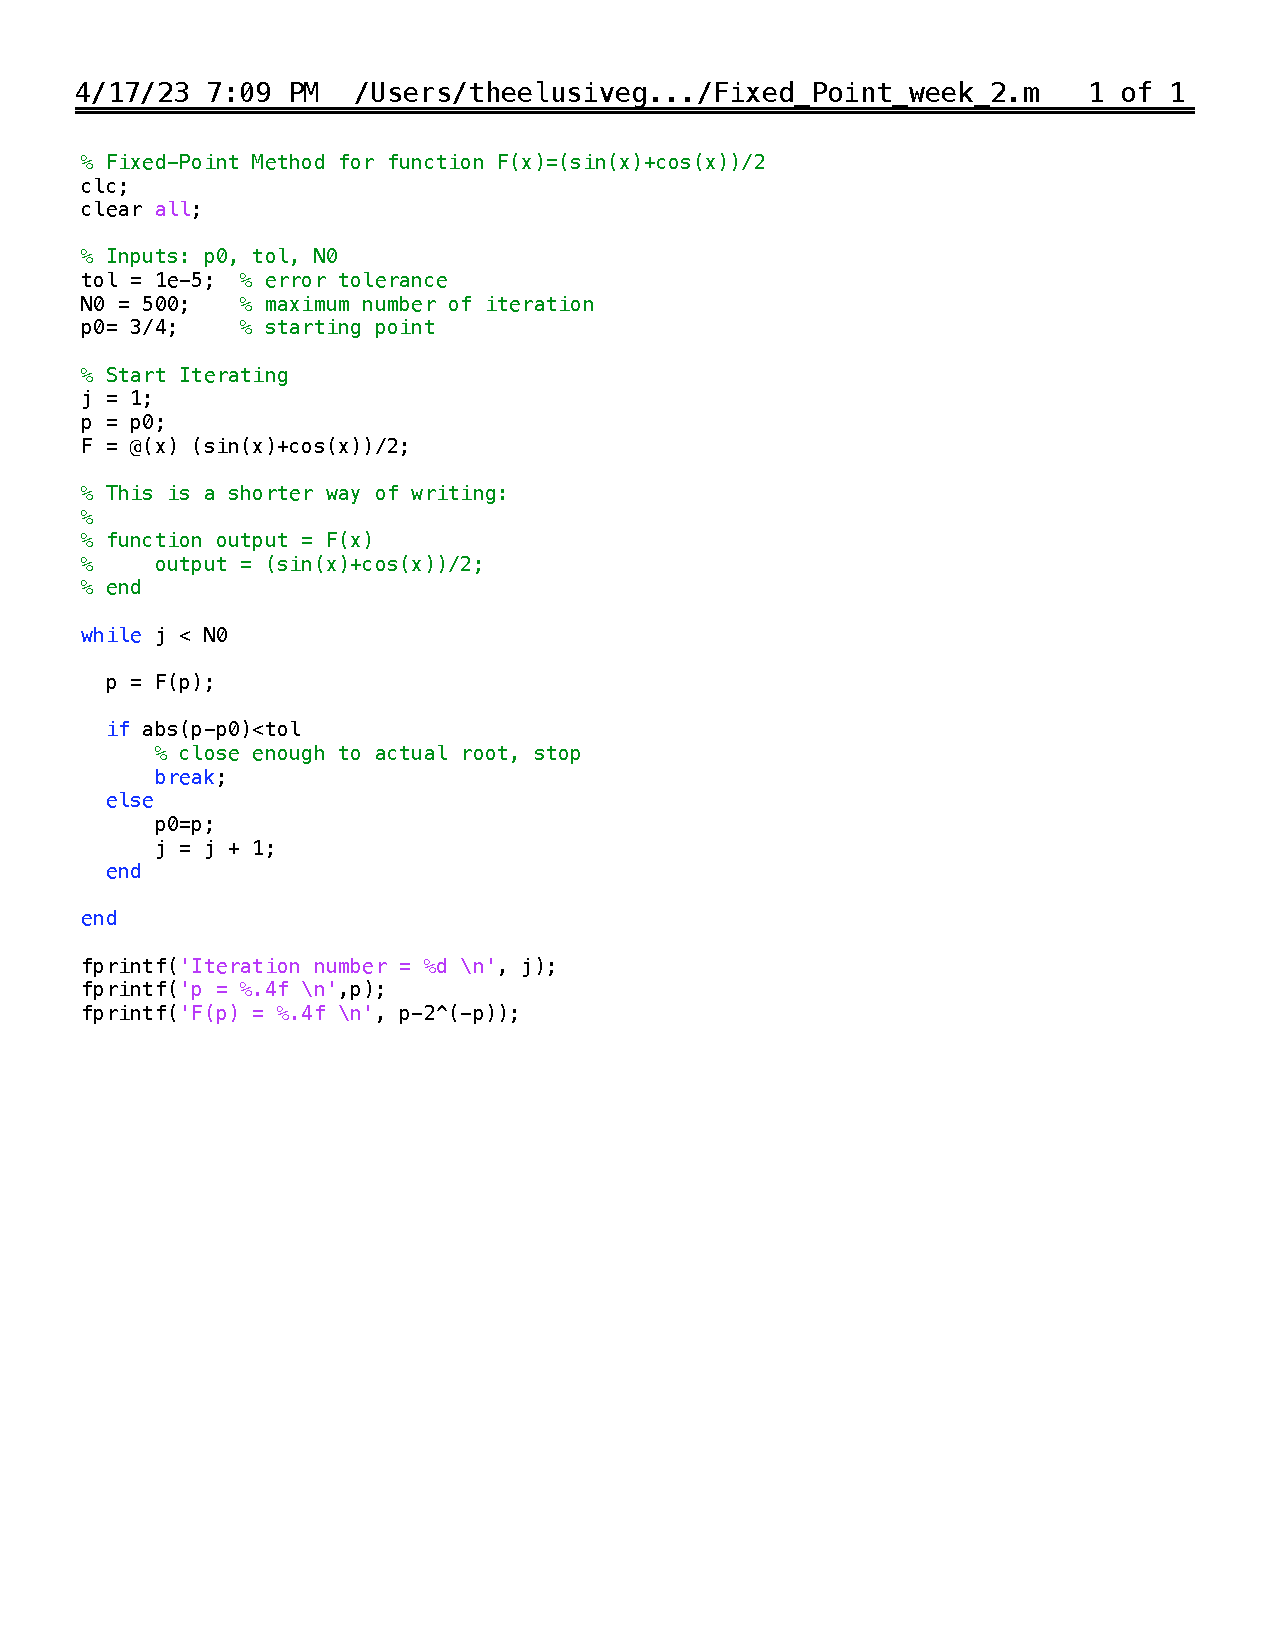
\includegraphics[width=\linewidth]{fixed_point_trig_1.pdf}  
    \end{minipage}%
    \begin{minipage}{.5\textwidth}
        \centering
        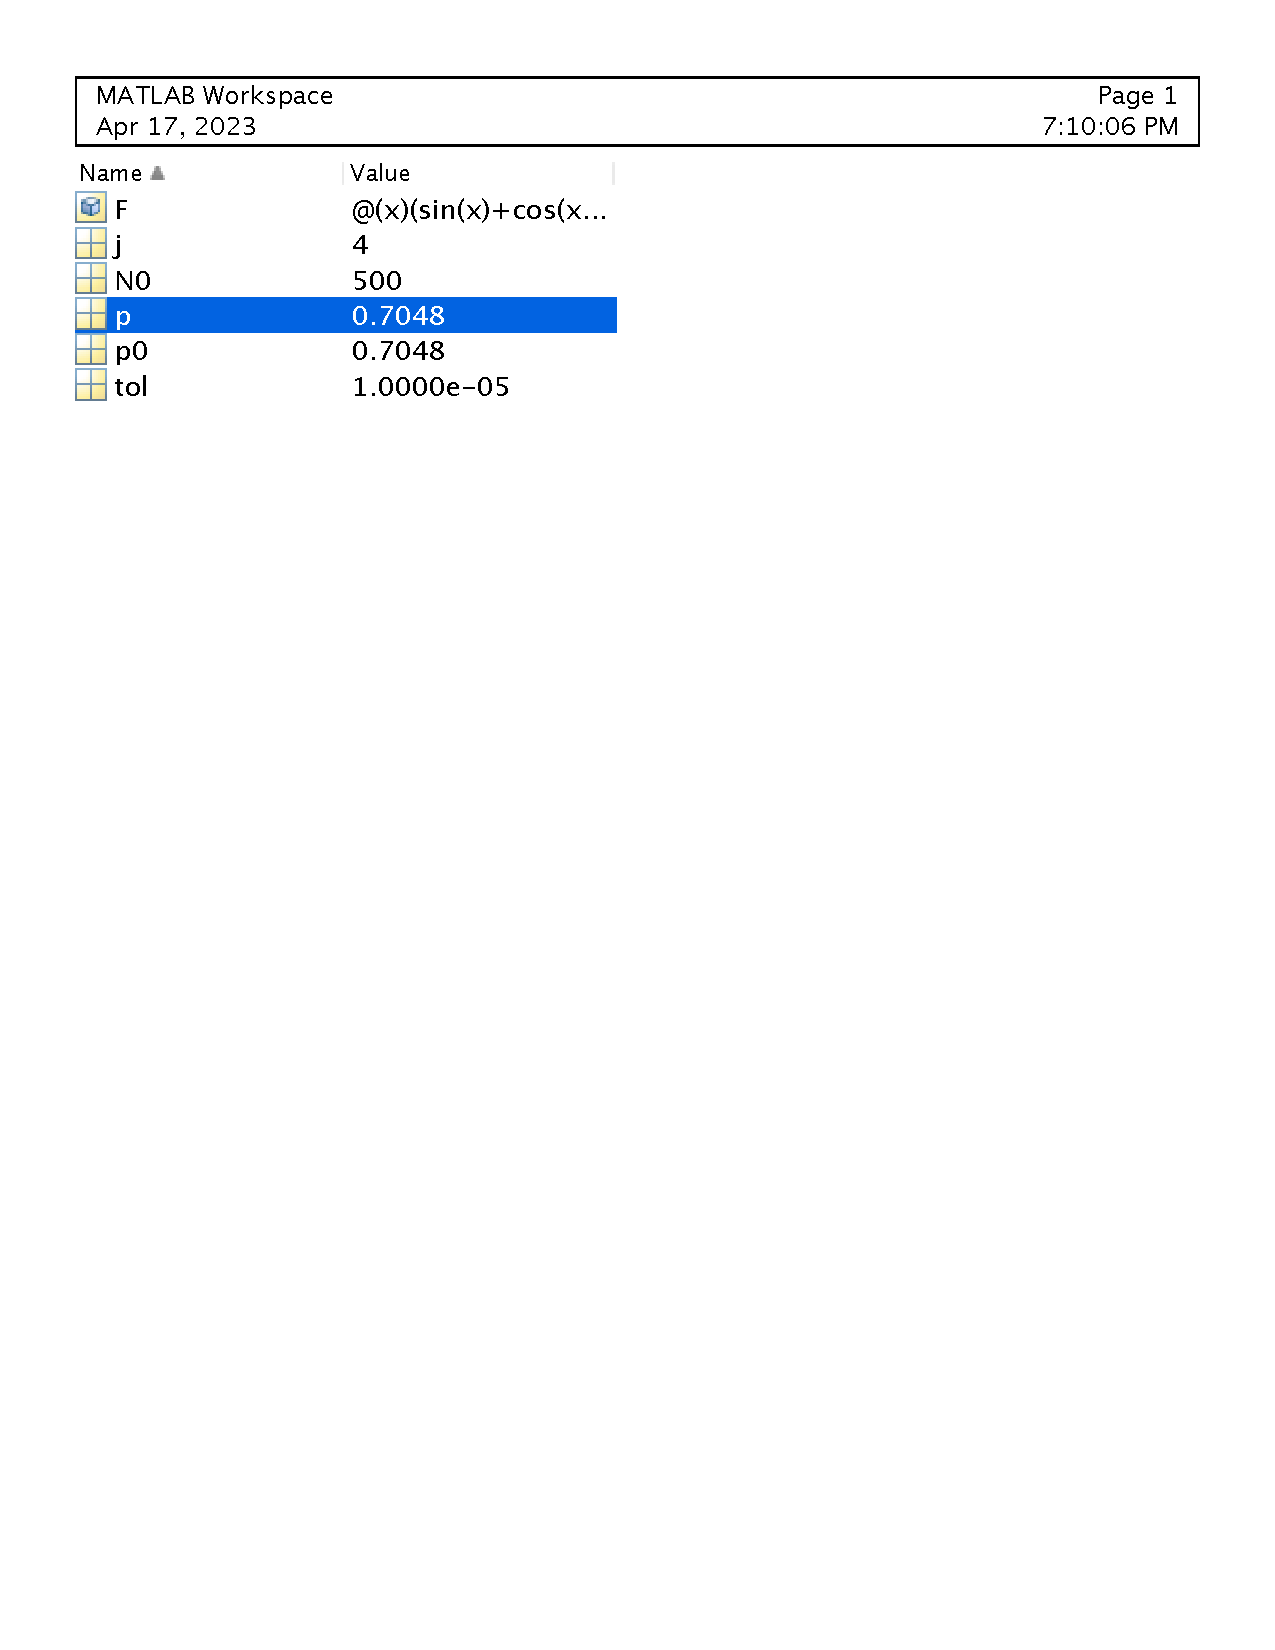
\includegraphics[width=\linewidth]{fix_point_workspace.pdf}
    \end{minipage}%
\end{figure}

\newpage
%%%%%%%%%%%%%%%%%%%%%%%%%%%%%%
\item \textbf{(T) A Toy Deep Network Problem}\\
Consider the iterative map $g(x)  = x -\frac{1}{3} \, \tanh(5\, x)$.
\begin{itemize} 
\item[a)]  Show that $g$ has a unique fixed point.

\item[b)]  Show that the FPM for this problem converges. 
\end{itemize}
\vspace{1em}
\textbf{Solution:}\par 
\begin{itemize} 
    \item[a)]  The maximum and minimum values of $g(x)$ for $x\in[-\frac{1}{4},\frac{1}{4}]$ must occur at the endpoints or when $g'(x)=0$.
    $g(x)$ assumes a maximum $g(-0.147)\approx0.0617$ and a minimum $g(0.147)\approx-0.0617$ when the derivative is 0.
    $[-0.0617,0.0617]\subset[-\frac{1}{4},\frac{1}{4}]$, so $g$ maps onto itself.
    Because $g$ is a continuous function that maps onto itself over the interval $[-\frac{1}{4},\frac{1}{4}]$, Theorem 2.3 states there exists a fixed point in the interval $[-\frac{1}{4},\frac{1}{4}]$.
    To show the fixed point is unique, we show $|g'(x)|$ is bounded above by a value $k$ less than 1.
    $|g'(x)|$ assumes a maximum at the endpoints $|g(0.25)|\approx0.5326$, so we set $k=0.5327$ which is less than 1.
    Because $|g'(x)|$ is bounded above by a constant less than 1, Theorem 2.3 states that the fixed point in $[-\frac{1}{4},\frac{1}{4}]$ is unique.
    \item[b)] The Fixed point Theorem states that if the conditions for Theorem 2.3 are satisfied, then for any $p_0\in[-\frac{1}{4},\frac{1}{4}]$ the sequence defined by $p_n=g(p_{n-1})$ converges to the unique fixed point in $[-\frac{1}{4},\frac{1}{4}]$.
\end{itemize}   
\newpage
%%%%%%%%%%%%%%%%%%%%%%%%%%%%%%
\item \textbf{(T) Fixed-Point Theory, One-sided Bound}
\begin{itemize} 
\item[a)] Prove the following: \\
``If $g \in C[a,b]$ and $g(x) \in [a,b]$ for all $x\in[a,b]$, then $g$ has a fixed-point in $[a,b]$. If, in addition, $g'(x)$ exists on $(a,b)$ and there exists a constant $K \in (0,1)$ with 
    $$g'(x) \leq K \ \ \text{for all} \ \  x\in[a,b],$$
    then the fixed-point is unique.''

For this problem, you do not need to write out the entire proof again, but you will need to indicate what parts should change and write down the new arguments.

\item[b)] Show that the theorem: \\
``Let $g \in C^1[a,b]$, i.e. $g'(x)$ exists on $(a,b)$, $g(x) \in [a,b]$ for all $x\in[a,b]$,  and there exists a $K \in (0,1)$ with 
    $$g'(x) \leq K \ \ \text{for all} \ \  x\in[a,b]$$
    then for any $p_0 \in [a,b]$ the sequence $p_n=g(p_{n-1})$ converges to the unique fixed-point $p\in [a,b]$ with $p=g(p)$.''\\
    does not hold by providing a counterexample. 

\textit{Hint: Show that $g(x)=1-x^2$ for $x\in[0,1]$ is a counterexample.}
\end{itemize}
\vspace{1em}
\textbf{Solution:}\par
\begin{itemize}
    \item [a)] Assume to the contrary $p$ and $q$ are distinct fixed points. 
    By the Mean Value Theorem, $\frac{g(q)-g(p)}{q-p}=\frac{q-p}{q-p}=g'(\xi_n)\le K<1$ for $\xi_n\in[a,b]$. 
    It follows that $q-p$=$g'(\xi_n)(q-p)$. This implies that $g'(\xi_n)=1$ or $p-q=0$. 
    Since $g'(\xi_n)\le K<1$ and $p$ and $q$ are distinct, it is impossible for either $g'(\xi_n)=1$ or $p-q=0$.
    Hence, we obtain a contradiction, so $p$ and $q$ can not be unique if $g'(x)<1$ for all $x\in[a,b]$.
    \item [b)] Let $g(x)=1-x^2$ for $x\in[0,1]$. 
    It follows $g'(x)=-2x\Rightarrow g'(x)<1$ for $x\in [0,1]$.
    If $p_0=1$ then $p_1=1\Rightarrow p_2=0...$$p_n=1$ for even n and $p_n=0$ for odd n (This is easily proven by induction).
    Because $p_n$ will osciliate between 2 values, it will not converge to the fixed point.
    
\end{itemize}
\newpage

%%%%%%%%%%%%%%%%%%%%%%%%%%%%%%
\item \textbf{(T) Fixed-Point Method for Lipschitz functions}\\
In this problem you will show that having a Lipschitz condition is sufficient for the fixed-point theory. 

\textbf{Definition:} A function $f:[a,b] \rightarrow \mathbb{R}$ is said to satisfy a \textit{Lipschitz condition} with Lipschitz constant $L>0$ on $[a,b]$ if, for every $x,y \in [a,b]$, we have $|f(x)-f(y)| \leq L |x-y|$. 


\begin{itemize} 
\item[a)] Prove the following:\par
``If $g \in C[a,b]$ and $g(x) \in [a,b]$ for all $x\in[a,b]$, then $g$ has a fixed-point in $[a,b]$. If, in addition, $g$ satisfies a Lipschitz condition on the interval $[a,b]$ with Lipschitz constant $L<1$, then the fixed-point is unique.''\par

For this problem, you do not need to write out the entire proof again, but you will need to indicate what parts should change and write down the new arguments.

 \vspace{0.5em}
\item[b)] Prove the following:\par 
``Let $g \in C^1[a,b]$, i.e. $g'(x)$ exists on $(a,b)$, $g(x) \in [a,b]$ for all $x\in[a,b]$,  and $g$ satisfies a Lipschitz condition on the interval $[a,b]$ with Lipschitz constant $L<1$, then for any $p_0 \in [a,b]$ the sequence $p_n=g(p_{n-1})$ converges to the unique fixed-point $p\in [a,b]$ with $p=g(p)$.''par

For this problem, you do not need to write out the entire proof again, but you will need to indicate what parts will change and write down the new arguments.


\end{itemize}

\vspace{1em}
\textbf{Solution:}\par
\begin{itemize}
    \item [a)] Assume to the contrary $p$ and $q$ are distinct fixed points. 
    Because $g$ satisfies a Lipschitz condition with $L<1$, $|p-q|=|f(p)-f(q)|\le L|p-q|$.
    It follows that for the innequality $|p-q|\le L|p-q|$ to hold, $L\ge1$ or $|p-q|=0$.
    Neither of these can be true because $L<1$ and $p$ and $q$ are distinct.
    Thus, we have a contradiction, so $f$ can only have one unique fixed point.   
    \item [b)] If $|p_n-p|=|f(p_{n-1})-f(p)|\le L|p_{n-1}-p|$, a simple induction $(|p_n-p|\le L|p_{n-1}-p|...\le L^{n-1}|p_1-p|\le L^n|p_0-p|)$ shows that $|p_n-p|\le L^n|p_0-p|$.
    $\displaystyle{\lim_{n\rightarrow\infty}}L^n|p_0-p|=0$ because $|L|<1$. 
    Taking the limit as $n$ goes to infinity of both sides shows that $\displaystyle{\lim_{n\rightarrow\infty}}|p_n-p|\le\displaystyle{\lim_{n\rightarrow\infty}}L^n|p_0-p|$ converges to $0$ by the Squeeze Theorem. 
\end{itemize}


\newpage
%%%%%%%%%%%%%%%%%
\item \textbf{(T) Fixed-Point Method}\\
Let $A$ be a given positive constant and define the fixed-point function $g(x)=2x-Ax^2$.
\begin{itemize} 
\item[a)] Verify that if the fixed-point algorithm (defined as $p_{n}=g(p_{n-1})$) converges to a non-zero limit, then the limit must be $p=\frac{1}{A}$.  (You should assume that $p_n \rightarrow p$ with $p>0$.)

\item[b)] Show that the fixed-point function satisfies $|g'(x)|<1$, only if $x \in (\frac{1}{2A}, \frac{3}{2A})$. 

(Note: This suggests that the largest interval of convergence that is guaranteed by the fixed-point theorem must be contained in $[\frac{1}{2A}, \frac{3}{2A}]$. The problem is that the interval is a function of the value $\frac{1}{A}$ which we are trying to calculate.)




\item[c)] Show that the fixed-point method converges to $\frac{1}{A}$ for any $p_0$  in $(0, \frac{2}{A})$ by proving  that $\left|p_n-\frac{1}{A} \right|  \leq k \left|p_{n-1}-\frac{1}{A} \right| $ for some $k \in (0,1)$.

(Note: This problem shows that any value $p_0$ close to but not equal to zero will lead to a convergent sequence. This is easier to use in practice.)
\end{itemize}
\vspace{1em}
\textbf{Solution:}\par
\begin{itemize}
    \item [a)] $\displaystyle{\lim_{n\rightarrow\infty}}p_n=\displaystyle{\lim_{n\rightarrow\infty}}g(p_n)=p=g(p)$. It follows, $p=2p-Ap^2\Rightarrow 0=p(p-\frac{1}{A})\Rightarrow p=0,\frac{1}{A}$. Thus if $p_n$ converges to a non-zero value, $p_n$ converges to $\frac{1}{A}$.
    \item [b)] $g'(x)=2-2Ax. If |g'(x)|<1$ then $-1<2-2Ax<1$. By subtracting $2$ and dividing by $-2A$, we obtain $\frac{1}{2A}<x<\frac{3}{2A}$. If $\frac{1}{2A}<x<\frac{3}{2A}$, then by multiplying by $-2A$ and adding $2$, we obtain $-1<2-2Ax<1\Rightarrow |2-2Ax|<1\Rightarrow |g'(x)|<1$. Because both directions hold, $|g'(x)|<1$ iff $-1<2-2Ax<1$.
    \item [c)] We want to show $|Ap_0-1|<1$ and $|p_n-\frac{1}{A}|\le |Ap_0-1||p_{n-1}-\frac{1}{A}|$ for any $p_0\in(0,\frac{2}{A})$\par
    First we show $|Ap_0-1|<1$. If $0<p_0<\frac{2}{A}\Rightarrow|p_0-\frac{1}{A}|<\frac{1}{A}\Rightarrow|Ap_0-1|<1$\par 
    Next we show $|p_n-\frac{1}{A}|=|Ap_{n-1}-1||p_{n-1}-\frac{1}{A}|$.\par
    $|p_n-\frac{1}{A}|=|g(p_{n-1})-\frac{1}{A}|=|2p_{n-1}-2A(p_{n-1})^2-\frac{1}{A}|=|A(p_{n-1}-\frac{1}{A})^2|=|Ap_{n-1}-1||p_{n-1}-\frac{1}{A}|$\par
    Next we want to show $|Ap_n-1|$ is a decreasing sequence and bounded above by some constant less than 1.\par
    $|Ap_n-1|=|A(2p_{n-1})-A(p_{n-1})^2)-1|=|2Ap_{n-1}-A^2p_{n-1}-1|=|(Ap_{n-1}-1)^2|$.\par
    Since $|Ap_0-1|<1$ and $|Ap_1-1|=|(Ap_0-1)^2|<|Ap_0-1|$, it follows by a simple induction $(|Ap_n-1|=|(Ap_{n-1}-1)^2|<|Ap_{n-1}-1|...<|Ap_1-1|=|(Ap_0-1)^2|<|Ap_0-1|<1)$.
    Thus $|Ap_n-1|$ is decreasing and bounded above by $|Ap_0-1|<1$\par 
    $|Ap_n-1|<|Ap_{n-1}-1|<|Ap_0-1|<1\Rightarrow |p_n-\frac{1}{A}|=|Ap_{n-1}-1||p_{n-1}-\frac{1}{A}|\le |Ap_0-1||p_{n-1}-\frac{1}{A}|$.\par 
    Hence, $|p_n-\frac{1}{A}|\le|Ap_0-1||p_{n-1}-\frac{1}{A}|$ where $|Ap_0-1|\in(0,1)$ for any $p_0\in(0,\frac{2}{A})$.\par
    $(|p_n-\frac{1}{A}|=|Ap_0-1|^{(2^n-1)}|p_0-\frac{1}{A}|)$ (more accurate equation for error. Not part of the solution).
\end{itemize}





\end{enumerate}

\end{document}


